\documentclass[11pt]{article}
\usepackage[utf8]{inputenc}
\usepackage{graphicx}
\usepackage{url}
% Load the package
\usepackage{glossaries}
 
% Generate the glossary
\makeglossaries

% Use wide margins, but not quite so wide as fullpage.sty
\marginparwidth 0.5in 
\oddsidemargin 0.25in 
\evensidemargin 0.25in 
\marginparsep 0.25in
\topmargin 0.25in 
\textwidth 6in \textheight 8 in


% multirow allows you to combine rows in columns
\usepackage{multirow}
% tabularx allows manual tweaking of column width
\usepackage{tabularx}
% longtable does better format for tables that span pages
\usepackage{longtable}

\begin{document}
\newglossaryentry{LHS}{name=LHS, description={Laboratoire à Haute Sécurité}}
\newglossaryentry{.dll}{name=DLL, description={Dynamic Link Library}}
\author{
Baptiste Decrand,						
Ndiasse Thioune,						
Alili Thanina,
Thibault Debonnière
\\[0.5cm]{\small Superviseur: Jean-Louis Lanet}
}

\title{Analyse Forensic de Malware \\Présentation du sujet}
\maketitle
\newpage
\section{Introduction}
\paragraph{}
Dans le cadre du mémoire à réaliser lors de la première année de Master Cryptis à l'université de Limoges, nous avons choisi le sujet Analyse Forensic de Malware proposé par le professeur Jean-Louis Lanet.

\paragraph{}
Ce projet consiste à étudier les malwares du type ransomware afin de créer une application qui permet d'identifier la classe du ransomware depuis une capture de l'image mémoire d'un système contaminé.


\section{Ransomware}
\paragraph{}
Le ransomware fait partie de la famille des malwares, c'est un logiciel malveillant apparu fin des années 80 qui est toujours d'actualité, on peut notamment cité le logiciel Wannacry qui a réussi à contaminer des grandes entreprises telles que Renault ou FedEx en mai 2017. Ces logiciels menacent l'utilisateur en bloquant l'accès aux données d'un système et obligent le propriétaire à payé une rançon afin de débloquer l'appareil infecté.
Il existe plusieurs types de ransomware, on peut les distinguer sur la manière qu'ils ont de chiffrer les données, en utilisant un chiffrement à clef asymétrique ou symétrique par exemple. Certains ransomwares ne chiffrent pas les données mais vont juste bloquer l'accès au système empêchant l'utilisateur peu expérimenté d'accéder à ces données. On peut aussi distinguer les ransomwares par le message de menace, en fonction du langage écrit ou bien de leurs contenus: certains sont des scarewares et se font passer pour des agences gouvernementales ou bien pour des antivirus.
\paragraph{}
Ces plans mémoires correspondent à un instant T de la mémoire, on peut alors récupérer plusieurs informations qui vont nous permettre de caractériser le ransomware tel que les noms d’API qui souhaite utiliser, les librairies (\gls{.dll}) utilisées, la page de rançon voir même les clefs de chiffrage. Cependant ces informations peuvent être incomplètes ou indisponibles en fonction de quand la capture a été faite, ce qui fait que chaque plan mémoire est unique et qu’on ne pourra se reposer sur un simple algorithme de pattern matching et qu'il faudra utiliser des algorithmes approchés afin de calculer le taux de ressemblance avec les familles de malwares.

\section{Application}
L'application que nous allons créer devra donc permettre à l'utilisateur de lui fournir une capture mémoire d'un ransomware et de récupérer des résultats qui lui permettront de savoir à quelle classe ce ransomware appartient.

Cette application sera composée de trois modules.
La première s’occupera d’extraire les données du dump mémoire sous forme de chaîne de caractères et devra filtrer les informations illisibles et inutiles afin de ne récupérer que les appels systèmes, les librairies utilisés et des informations spécifiques.
Une fois ces données récupérées, elles seront transformées en vecteurs binaires et seront soumises à huit métriques.
Ces métriques devront calculer la distance et la similarité avec des familles définies de ransomware.
Le troisième module sera une interface graphique qui permettra de visualiser et de mettre en avant les résultats obtenus ainsi que les informations importantes du ransomware (famille du ransomware, page de rançon ou serveur associé, clé de chiffrage, etc.).

Pour réaliser ces comparaissons, nous disposons grâce aux \gls{LHS} de Rennes d'une base de données de plan mémoire (dump de binaires dépaquetés) de ransomware dont on connaît pour une partie à quelles classes ils appartiennent. Ces derniers serviront d'une base d'apprentissage afin de tester le bon fonctionnement de notre programme.

\begin{figure}[h]
  \centering
  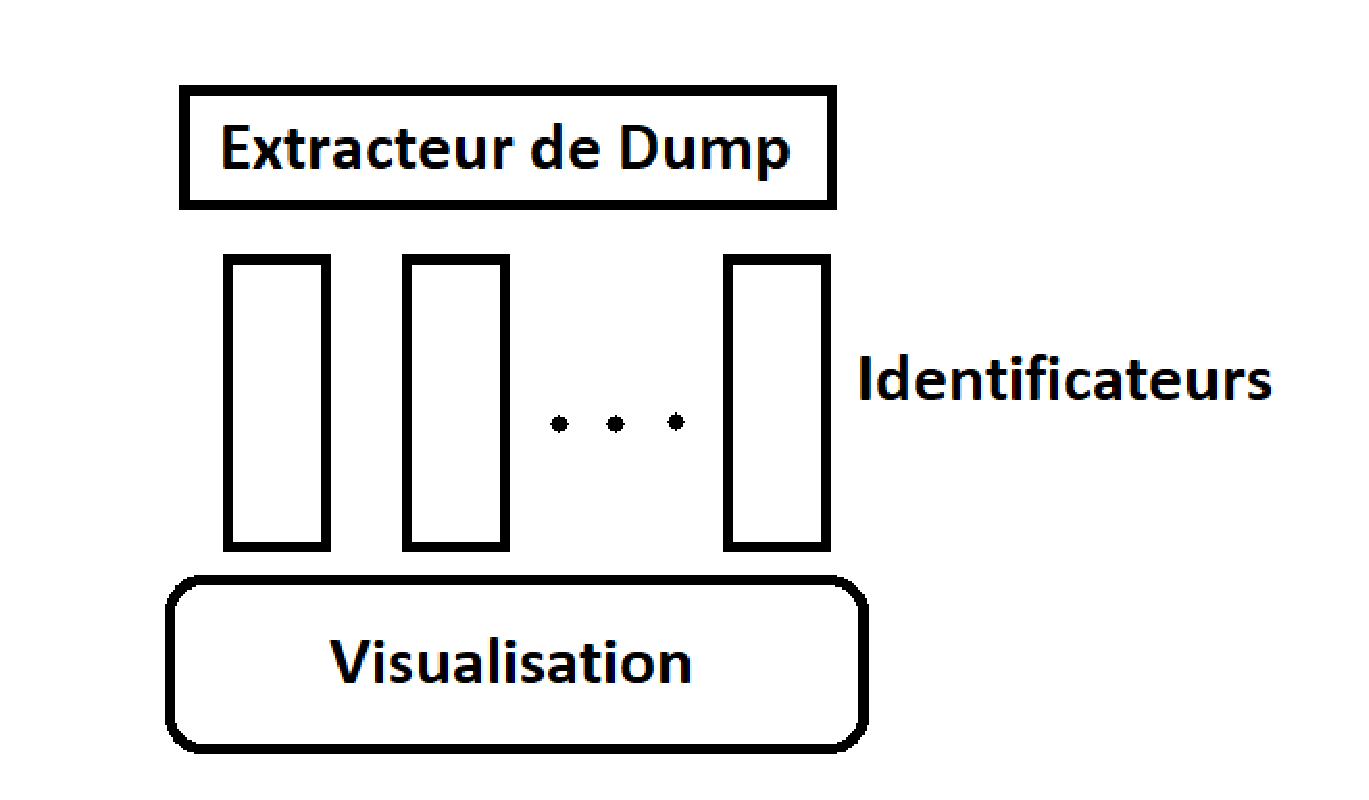
\includegraphics[scale=0.40]{unknown.eps}
  \caption{Schémas de l'application}
\end{figure}

Lors du premier semestre, nous réaliserons un prototype de notre logiciel avec la lecture du dump mémoire, une métrique et l’interface graphique. Un premier mémoire sera rédigé sur nos recherches sur le sujet, les algorithmes utilisés, nos choix d’implémentation, les contraintes rencontrées ainsi que la manière dont on s’est organisé (Support, répartition des tâches etc).
Le second semestre nous permettra d’implémenter les autres métriques et d’améliorer notre logiciel afin de pouvoir le présenter une soutenance qui se déroulera vers les vacances de Pâques. Nous rendrons notre mémoire qui complétera le premier avec notre travail lors de ce second semestre. 

\section{Métriques}
Nous allons implémenter huit métriques dans l'application, celles-ci détermineront la distance ou la similitude entre deux vecteurs binaires.

Une fonction de similitude renverra 0 si les deux vecteurs sont égaux et tendra vers l'infini la dissimilarité.Une fonction de distance renverra une valeur entre 0 et 1, 1 représentant l'égalité des deux vecteurs.

Un vecteur binaire sera construit de telle manière que la présence d'une chaîne de caractères d'un appel système ou d'une librairie sera représenté par un 1 et l'absence par un zéro.

Les vecteurs binaires de comparaison qui représenteront les familles de ransomware seront construit depuis une base de données contenant des captures mémoire de ransomware connu.

Soit A et B deux vecteurs binaires de taille $n$.

On définit:

   $n_{A0}$, la quantité de 0 du vecteur A.
   
   $n_{A1}$, la quantité de 1 du vecteur A.
    
   $S0_{A}0_{B}$, le nombre de couple (0,0) pour les vecteurs binaires X,Y quand $A_{i} = 0$ et $B_{i} = 0$.

   $S1_{A}0_{B}$, le nombre de couple (1,0) pour les vecteurs binaires X,Y quand $A_{i} = 1$ et $B_{i} = 0$.

   $S0_{A}1_{B}$, le nombre de couple (0,1) pour les vecteurs binaires X,Y quand $A_{i} = 0$ et $B_{i} = 1$.

   $S1_{A}1_{B}$, le nombre de couple (1,1) pour les vecteurs binaires X,Y quand $A_{i} = 1$ et $B_{i} = 1$.\\
   


\subsection{Similarité de Cosine}
Le calcul de la similarité de Cosine s'obtient par le rapport entre le produit scalaire et le produit de la norme des vecteurs.

\[
    S = \frac{A \cdot B}{||A|| \cdot ||B||}
    \Leftrightarrow S = \frac{\sum_{i=0}^n A_{i}B_{i}}{\sqrt{\sum_{i=0}^n A_{i}}\times\sqrt{\sum_{i=0}^n B_{i}}}
    \Leftrightarrow S = \frac{S1_{A}S1_{B}}{\sqrt{n_{A1}}\times \sqrt{n_{B1}}}
\]\\
Après cette simplification, on remarque que la similarité de Cosine se base uniquement sur la présence de chaîne de caractères, et constitue donc le rapport entre la présence commune de chaînes et le produit de la quantité de présence de chaque vecteurs.
\subsection{Distance de Hamming}
La distance de Hamming peut être définie comme un quantificateur capable de faire la différence entre deux séquences de symboles de même longueur.
Le principe de la distance de Hamming consiste à comparer les caractères les uns à la suite des autres.
Il faut calculer le nombre de bits qui sont différents entre deux vecteurs binaires, c’est à dire pour deux séquences de caractères x et y , on parcourt toutes les caractères de x et de y , puis on regarde si la valeur de x et de y sont identiques dans toutes les colonnes , si oui on divise le nombre de (x,y) similaires présent dans le vecteur avec la taille du vecteur N. 

On peut l’illustrer par le formule suivant:

\begin{equation}
   H = \frac{S1_{A}1_{B}+S0_{A}0_{B}}{S1_{A}1_{B} + S0_{A}1_{B}+S1_{A}0_{B} + S0_{A}0_{B}}
\end{equation}


\subsection{Distance de Kulzinsky}
\paragraph{}
La distance de Kulzinsky se base sur la probabilité conditionnelle que la caractéristique est présente dans un élément, pour peu qu'elle soit présente dans l'autre. Les valeurs distinctes pour chaque élément agissant comme prédicteur de l'autre sont considérées par leur moyenne pour calculer cette valeur.

Le coefficient de similarité est calculé par :
\begin{equation}
   D = \frac{S1_{A}1_{B}}{S1_{A}0_{B} + S0_{A}1_{B}}
\end{equation}

\subsection{Distance de Sokal et Sneath}
\paragraph{}
L'indice de Sokal et Sneath 
\paragraph{}
\'{E}tant donné deux objets A et B, chacun avec n attributs binaires, l’indice se calcule de la manière qui suit :

\begin{equation}
   D = \frac{2\times(S0_{A}0_{B}+S1_{A}1_{B})}{2\times(S0_{A}0_{B} + S1_{A}1_{B})+S1_{A}0_{B} + S0_{A}1_{B}}
\end{equation}

\subsection{Distance de Jaccard}

L'indice de Jaccard est le rapport entre le nombre d'éléments sur le total du nombre d'élément. Formalisé comme ceci :
\begin{equation}
   J( A, B)= \frac{|A \cap B|}{|A \cup B|}
\end{equation}

Plus concrètement, on obtient l'indice de Jaccard avec cette relation :

\begin{equation}
  J =\frac{ S1_{A}1_{B} }{S0_{A}1_{B}+S1_{A}0_{B}+S1_{A}1_{B}}
\end{equation}
\textit{Note : La distance de Jaccard correspond à l'opposé de cette formule.}
\\


On remarque que l'indice de Jaccard n'est en fait qu'un simple calcul du ratio entre les éléments communs et les élément différents de nos 2 ensembles. MAIS sans tenir compte de $S0_{A}0_{B}$. Donc l'indice de Jaccard considérera les éléments non utilisés dans les deux ensembles comme des différences(contrairement à la distance de Hamming).




\subsection{Distance Euclidienne}

On définit la distance Euclidienne de la façon suivante :
\begin{equation}
 \sqrt{\sum_{i=0}^n (A_{i}-B_{i})^2}
\end{equation}

La distance Euclidienne n'est en fait qu'un simple "compteur de différence" qui va s'incrémenter à chaque différence nette entre 2 éléments. En effet, la distance euclidienne peut se simplifier comme ceci :

\begin{equation}
 \sqrt{S1_{A}0_{B}+S1_{A}0_{B}}
\end{equation}

On obtient un résultat absolu que l'on va relativiser en divisant par le nombre d'éléments.

\subsection{Distance de Russel-Rao}
La distance de Russel-and-Rao est une métrique qui se calcule grâce au nombre de 1 que les deux séquences  de vecteurs binaires partagent dans les mêmes positions, par rapport au nombre total de 1 dans la première séquence, le nombre total de 1 que les deux vecteurs partagent sera ensuite divisé par la taille du vecteur N.  Si une variable est comparée à elle-même, il peut être nécessaire que la similitude soit égale à la valeur 1.
La définition est la suivante :
\begin{equation}
   RR = \frac{S1_{A}1_{B}}{S1_{A}1_{B} + S0_{A}1_{B}+S1_{A}0_{B} + S0_{A}0_{B}}
\end{equation}

\subsection{Distance de Anderberg}
La distance de Anderberg est donné par la formule:
\begin{equation}
   D = \frac{S1_{A}1_{B}}{S1_{A}1_{B} + 2\times(S1_{A}0_{B}+S0_{A}1_{B})}
\end{equation}
Le calcul de cette distance met en avant la disparité des vecteurs lorsqu'une chaîne de caractère est uniquement présente dans l'un d'entre eux. En effet la distance est divisée par deux fois le nombres de chaînes non commune. Cette distance ne prend pas en compte le fait que des chaînes ne sont pas présentes dans les deux vecteurs ($S0_{A}S0_{B}$).

\subsection{Comparaison}


Soit le couple X,Y
\[
   X = \{0,1,1,1,0,0,1,1,0,1\}
\]
\[
  Y = \{0,0,0,1,1,1,0,0,1,1\} 
\]
\[
S0_{A}0_{B}=1 \qquad
S0_{A}1_{B}=3 \qquad
S1_{A}0_{B}=4 \qquad
S1_{A}1_{B}=2
\]

Et le couple U,V
\[
   U = \{1,0,1,0,0,1,1,0,1,0,0,0,1,0,1,0,1,0,1,1\}
\]
\[
   V = \{0,1,0,1,1,0,1,0,1,0,0,1,0,1,0,1,1,0,0,1\}
\]
\[
S0_{A}0_{B}=4  \qquad
S0_{A}1_{B}=6  \qquad
S1_{A}0_{B}=6  \qquad
S1_{A}1_{B}=4
\]
\\
Calculons selon les deux couples de vecteur (X,Y) et (U,V), les huit métriques

\begin{tabular}{|l|l|l|}
    \hline
   Métriques & $\{X,Y\}$ & $\{U,V\}$\\
   \hline
   Cosine & 0.365 & 0.040\\
   \hline
   Sokal et Sneath & ? & ?\\
   \hline
   Kulzinsky & 0.333 & 0.333\\
   \hline
   Hamming & 0.333 & 0.400\\
   \hline
   Jaccard & 0.222 & 0.286\\
   \hline
   Euclidienne & 0.264 & 0.173\\
   \hline
   Russel-Rao & 0.200 & 0.400\\
   \hline
   Anderberg & 0.125 & 0.143\\
   \hline
\end{tabular}\\

\begin{itemize}
\item Hamming et Jaccard deux formules semblables, à la différence que Hamming considérera les éléments absents dans les deux ensembles comme des points communs, alors que Jaccard le fait comme des différences. Ce qui n'est pas optimale dans notre cas.

\end{itemize}


\section{Conclusion}
Ce sujet nous permettra d'étudier le fonctionnement des ransomwares et leurs spécificités. Ce projet aboutira sur une application capable de classer les ransomwares ce qui sera une manière concrète de montrer nos connaissances et notre implication au cours de ce semestre.



\newpage
Lien vers le dépôt de fichiers git

\url{https://git.unilim.fr/decrand1/AnalyseRansomware}

\printglossaries
 
 \end{document}
